\documentclass[10pt,t]{beamer}

\input{mypreamble}

\title{Introduction to OpenACC}
\subtitle{2017~HPC~Workshop:~Parallel~Programming}
\author{\large{Alexander~B.~Pacheco}}
\institute{\href{http://researchcomputing.lehigh.edu}{LTS Research Computing}}
\date{May~31~-~June~1,~2017}
    

\begin{document}

\begin{frame}
  \titlepage
\end{frame}

\scriptsize
\begin{frame}{ What is OpenACC?}
  \begin{block}{}
    \begin{itemize}
      \item OpenACC Application Program Interface describes a collection of compiler directive to specify loops and regions of code in standard C, C++ and Fortran to be offloaded from a host CPU to an attached accelerator.
      \item provides portability across operating systems, host CPUs and accelerators
    \end{itemize}
  \end{block}
\end{frame}

\begin{frame}[allowframebreaks]{\small OpenACC}
  \begin{exampleblock}{The Standard for GPU Directives}
    \begin{description}
      \item[Simple:] Directive are the easy path to accelerate compute intensive applications
      \item[Open:] OpenACC is an open GPU directives standard, making GPU programming straightforwards and portable across parallel and multi-core processors
      \item[Powerful:] GPU directives allow complete access to the massive parallel power of a GPU
    \end{description}
  \end{exampleblock}
  \framebreak
  \begin{exampleblock}{High Level}
    \begin{itemize}
      \item Compiler directives to specify parallel regions in C \& Fortran
      \begin{itemize}
        \item Offload parallel regions
        \item Portable across OSes, host CPUs, accelerators, and compilers
      \end{itemize}
      \item Create high-level heterogenous programs
      \begin{itemize}
        \item Without explicit accelerator intialization
        \item Without explicit data or program transfers between host and accelerator
      \end{itemize}
    \end{itemize}
  \end{exampleblock}
  \begin{exampleblock}{High Level $\cdots$ with low-level access}
    \begin{itemize}
      \item Programming model allows programmers to start simple
      \item Compiler gives additional guidance
      \begin{itemize}
        \item Loop mappings, data location and other performance details
      \end{itemize}
      \item Compatible with other GPU languages and libraries
      \begin{itemize}
        \item Interoperate between CUDA C/Fortran and GPU libraries
        \item e.g. CUFFT, CUBLAS, CUSPARSE, etc
      \end{itemize}
    \end{itemize}
  \end{exampleblock}
\end{frame}

\begin{frame}{ Why OpenACC}
  \begin{exampleblock}{}
    \begin{itemize}
      \item Directives are easy and powerful.
      \item Avoid restructuring of existing code for production applications.
      \item Focus on expressing parallelism.
    \end{itemize}
  \end{exampleblock}
  \vspace{1cm}
  \begin{alertblock}{}
    \begin{center}
      \vspace{0.1cm}
      \Large{\color{red!80!black}OpenACC is not GPU Programming}\\
      \vspace{1cm}
      \Large{\color{red!80!black}OpenACC is Expressing Parallelism in your code}
    \end{center}
  \end{alertblock}
\end{frame}

\begin{frame}{Exercises:}
  \begin{itemize}
    \item Recall the following three exercises from yesterday's OpenMP tutorial
    \begin{enumerate}
      \item SAXPY: Generalized vector addition
      \item Matrix Multiplication
      \item Calculate pi by Numerical Integration
    \end{enumerate}
  \end{itemize}
\end{frame}

\begin{frame}{ SAXPY}
  \begin{itemize}
    \item SAXPY is a common operation in computations with vector processors included as part of the BLAS routines
    \item[] $y\leftarrow \alpha x + y$
%    \item SAXPY is a combination of scalar multiplication and vector addition
    \item Write a SAXPY code to multiply a vector with a scalar.
  \end{itemize}
  \begin{algorithm}[H]
    \caption{Pseudo Code for SAXPY}
    \begin{algorithmic}
      \Program{saxpy}{}
      \State $n \gets$ some large number
      \State $x(1:n) \gets$ some number say, 1
      \State $y(1:n) \gets$ some other number say, 2
      \State $a \gets$ some other number ,say, 3
      \Do{$i \gets 1\cdots n$}
      \State $y_i \gets y_i + a * x_i$
      \EndDo
      \EndProgram{saxpy}
    \end{algorithmic}
  \end{algorithm}
\end{frame}

\begin{frame}[allowframebreaks]{Matrix Multiplication}
  \begin{itemize}
    \item Most Computational code involve matrix operations such as matrix multiplication.
    \item Consider a matrix {\bf C} which is a product of two matrices {\bf A} and {\bf B}:
    \item[] Element {\it i,j} of {\bf C} is the dot product of the $i^{th}$ row of {\bf A} and $j^{th}$ column of {\bf B}
    \item Write a MATMUL code to multiple two matrices.
  \end{itemize}
  \begin{center}
    \includegraphics[width=0.5\textwidth]{./matmul}
  \end{center}

  \begin{algorithm}[H]
    \caption{Pseudo Code for MATMUL}
    \begin{algorithmic}
      \Program{matmul}{}
      \State $m,n \gets$ some\,large\,number $\le 1000$
      \State Define $a_{mn}, b_{nm}, c_{mm}$
      \State $a_{ij} \gets i+j; b_{ij} \gets i-j; c_{ij} \gets 0$
      \Do{$i \gets 1\cdots m$}
      \Do{$j \gets 1\cdots m$}
      \State $c_{i,j} \gets \sum^{n}_{k=1} a_{i,k}*b_{k,j}$
      \EndDo
      \EndDo
      \EndProgram{matmul}
    \end{algorithmic}
  \end{algorithm}
\end{frame}

\begin{frame}[allowframebreaks]{Calculate pi by Numerical Integration}
  \begin{columns}
    \column{5cm}
    \begin{itemize}
      \item We know that
      \begin{align*}
        \int^1_0 \dfrac{4.0}{(1+x^2)}\, dx = \pi
      \end{align*}
      \item So numerically, we can approxiate pi as the sum of a number of rectangles
      \begin{align*}
        \sum^N_{i=0}\,F(x_i)\Delta x \approx \pi
      \end{align*}
      \item[] \fontsize{4}{5}{ Meadows et al, A ``hands-on'' introduction to OpenMP, SC09 }
    \end{itemize}
    \column{5cm}
    \begin{center}
      \includegraphics[width=4cm]{./pi}
    \end{center}
  \end{columns}

  \begin{algorithm}[H]
    \caption{Pseudo Code for Calculating Pi}
    \begin{algorithmic}
        \Function{calculate\_pi}{}
        \State $step \gets 1/n$
        \State $sum \gets 0$
        \Do{$i \gets 0\cdots n$}
        \State $x \gets (i+0.5)*step; sum \gets sum + 4/(1+x^2)$
        \EndDo
        \State $pi \gets sum * step$
        \EndFunction
    \end{algorithmic}
  \end{algorithm}
\end{frame}

\begin{frame}[fragile]{\small Simple Example {\color{black}I}}
  \begin{exampleblock}{Serial Code}
    \lstinputlisting[basicstyle=\fontsize{5}{6}\selectfont\ttfamily,language=OmpFortran]{./src/saxpy/solution/saxpy.f90} 
  \end{exampleblock}
\end{frame}
\begin{frame}[fragile]{\small Simple Example {\color{black}II}}
  \begin{exampleblock}{OpenMP Code}
    \lstinputlisting[basicstyle=\fontsize{5}{6}\selectfont\ttfamily,language=OmpFortran]{./src/saxpy/solution/saxpy_omp.f90} 
  \end{exampleblock}
\end{frame}
\begin{frame}[fragile]{\small Simple Example {\color{black}III}}
  \begin{exampleblock}{OpenACC Code}
    \lstinputlisting[basicstyle=\fontsize{5}{6}\selectfont\ttfamily,language=OmpFortran]{./src/saxpy/solution/saxpy_acc.f90} 
  \end{exampleblock}
\end{frame}
\begin{frame}[fragile]{\small Simple Example {\color{black}IV}}
  \begin{exampleblock}{CUDA Fortran Code}
    \lstinputlisting[basicstyle=\fontsize{5}{6}\selectfont\ttfamily,language=OmpFortran]{./src/saxpy/solution/saxpy_cuda.f90} 
  \end{exampleblock}
\end{frame}

\begin{frame}[fragile]{\small Simple Example {\color{black}V}}
  \begin{exampleblock}{Compile}
    {\tiny
      \begin{Verbatim}
[apacheco@mike1 2013-LONI]$ pgf90 -o saxpy saxpy.f90
[apacheco@mike1 2013-LONI]$ pgf90 -mp -o saxpy_omp saxpy_omp.f90
[apacheco@mike1 2013-LONI]$ pgf90 -acc -ta=nvidia -o saxpy_acc saxpy_acc.f90
[apacheco@mike1 2013-LONI]$ pgf90 -o saxpy_cuda saxpy.cuf
      \end{Verbatim}
    }
  \end{exampleblock}
  \begin{exampleblock}{Speed Up}
    \begin{center}
      \begin{tabular}{|bbbb|}
        \hline
        \rowcolor{lublue}Algorithm & Device & Time (s) & Speedup \\
        \hline
        Serial & Xeon E5-2670 & 0.986609 & 1\\
        OpenMP (8 threads) & Xeon E5-2670 & 0.241465 & 4.1x\\
        OpenACC & M2090 & 0.059418 & 16.6x\\
        CUDA & M2090 & 0.005205 & 189.5x\\
        \hline
      \end{tabular}
    \end{center}
  \end{exampleblock}
\end{frame}

\begin{frame}{ OpenACC Execution Model}
  \begin{exampleblock}{}
    \begin{itemize}
      \item Application code runs on the CPU (sequential, shared or distributed memory)
      \item OpenACC directives indicate that the following block of compute intensive code needs to be offloaded to the GPU or accelerator.
    \end{itemize}
    \vspace{-0.5cm}
        \begin{center}
      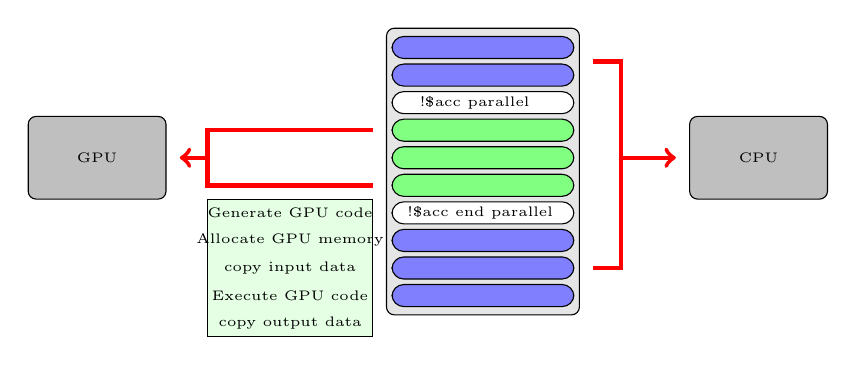
\begin{tikzpicture}[scale=0.35]
        \tikzstyle{every node}=[font=\tiny]
        \filldraw[fill=gray!20!white,rounded corners=1mm] (0,-0.2) rectangle (7,10.2);
        \filldraw[fill=blue!50!white,rounded corners=1.5mm] (0.2,0.1) rectangle (6.8,0.9);
        \filldraw[fill=blue!50!white,rounded corners=1.5mm] (0.2,1.1) rectangle (6.8,1.9);
        \filldraw[fill=blue!50!white,rounded corners=1.5mm] (0.2,2.1) rectangle (6.8,2.9);
        \filldraw[fill=white,rounded corners=1.5mm] (0.2,3.1) rectangle (6.8,3.9);
        \filldraw[fill=green!50!white,rounded corners=1.5mm] (0.2,4.1) rectangle (6.8,4.9);
        \filldraw[fill=green!50!white,rounded corners=1.5mm] (0.2,5.1) rectangle (6.8,5.9);
        \filldraw[fill=green!50!white,rounded corners=1.5mm] (0.2,6.1) rectangle (6.8,6.9);
        \filldraw[fill=white,rounded corners=1.5mm] (0.2,7.1) rectangle (6.8,7.9);
        \filldraw[fill=blue!50!white,rounded corners=1.5mm] (0.2,8.1) rectangle (6.8,8.9);
        \filldraw[fill=blue!50!white,rounded corners=1.5mm] (0.2,9.1) rectangle (6.8,9.9);
        \draw (3.4,3.5) node {!\$acc end parallel};
        \draw (3.2,7.5) node {!\$acc parallel};
        \draw[ultra thick,red] (7.5,1.5) -- (8.5,1.5) -- (8.5,9.0) -- (7.5,9.0);
        \draw[->,ultra thick,red] (8.5,5.5) -- (10.5,5.5);
        \draw[ultra thick,red] (-0.5,4.5) -- (-6.5,4.5) -- (-6.5,6.5) -- (-0.5,6.5);
        \draw[->,ultra thick,red] (-6.5,5.5) -- (-7.5,5.5);
        \filldraw[fill=gray!50!white,rounded corners=1mm] (-8.0,4.0) rectangle (-13.0,7,0);
        \filldraw[fill=gray!50!white,rounded corners=1mm] (11.0,4.0) rectangle (16.0,7,0);
        \draw (-10.5,5.5) node {GPU};
        \draw (13.5,5.5) node {CPU};
        \filldraw[fill=green!10!white] (-6.5,-1.0) rectangle (-0.5,4.0);
        \draw (-3.5,3.5) node {Generate GPU code};
        \draw (-3.5,2.5) node {Allocate GPU memory};
        \draw (-3.5,1.5) node {copy input data};
        \draw (-3.5,0.5) node {Execute GPU code};
        \draw (-3.5,-0.5) node {copy output data};
      \end{tikzpicture}
      \vspace{-0.8cm}
    \end{center}

  \end{exampleblock}
\end{frame}

\begin{frame}[fragile]
  \frametitle{\small Building Block of OpenACC}
  \begin{itemize}
  \item Program directives
    \begin{itemize}
    \item Syntax
      \begin{itemize}
      \item C/C++: \Verbred{\#pragma acc <directive> [clause]}
      \item Fortran: \Verbred{!\$acc <directive> [clause]}
      \end{itemize}
    \item Regions
    \item Loops
    \item Synchronization
    \item Data Structure
    \item $\cdots$
    \end{itemize}
  \item Runtime library routines
%      \item Environment variables
  \end{itemize}
\end{frame}

\begin{frame}[fragile]{\small Clauses}
  \begin{itemize}
    \item \Verbred{if (condition)}
    \item \Verbred{async (expression)}
    \item data management clauses
    \begin{itemize}
      \item \Verbred{copy($\cdots$),copyin($\cdots$), copyout($\cdots$)}
      \item \Verbred{create($\cdots$), present($\cdots$)}
      \item \Verbred{present\_or\_copy\{,in,out\}($\cdots$)} or \Verbred{pcopy\{,in,out\}($\cdots$)}
      \item \Verbred{present\_or\_create($\cdots$)} or \Verbred{pcreate($\cdots$)}
    \end{itemize}
    \item \Verbred{reduction(operator:list)}
  \end{itemize}
\end{frame}

\begin{frame}[fragile]{\small Runtime Libraries}
  \begin{itemize}
    \item System setup routines
    \begin{itemize}
      \item \Verbred{acc\_init(acc\_device\_nvidia)}
      \item \Verbred{acc\_set\_device\_type(acc\_device\_nvidia)}
      \item \Verbred{acc\_set\_device\_num(acc\_device\_nvidia)}
    \end{itemize}
    \item Synchronization routines
    \begin{itemize}
      \item \Verbred{acc\_async\_wait(int)}
      \item \Verbred{acc\_async\_wait\_all()}
    \end{itemize}
  \end{itemize}
\end{frame}

%\begin{frame}<0>{\small Environment Variables}
%  \begin{itemize}
%    \item OMP\_NUM\_THREADS
%    \item OMP\_SCHEDULE
%    \item OMP\_STACKSIZE
%    \item OMP\_DYNAMIC
%    \item OMP\_NESTED
%    \item OMP\_WAIT\_POLICY
%    \item more $\cdots$
%  \end{itemize}
%\end{frame}

\begin{frame}[fragile]{\small OpenACC kernels directive}
  \begin{columns}
    \column{0.6\textwidth}
    \begin{itemize}
      \item[C:] \Verbred{\#pragma acc kernels [clause]}
      \item[Fortran] \Verbred{!\$acc kernels [clause]}
      \item The kernels directive expresses that a region may contain parallelism and the compiler determines what can be safely parallelized.
      \item The compiler breaks code in the kernel region into a sequence of kernels for execution on the accelerator device.
      \item For the codes on the right, the compiler identifies 2 parallel loops and generates 2 kernels.
      \item {\color{red}What is a kernel?} {\color{DarkGreen}A function that runs in parallel on the GPU.}
      \item When a program encounters a kernels contruct, it will launch a sequence of kernels in order on the device.
    \end{itemize}
    \column{0.3\textwidth}
    \begin{exampleblock}{}
      \lstinputlisting[basicstyle=\tiny\ttfamily,language=OmpFortran,firstline=98,lastline=107]{src/tmp.f90}
      \lstinputlisting[basicstyle=\tiny\ttfamily,language=OmpC,firstline=50,lastline=60]{src/tmp.c}
    \end{exampleblock}
  \end{columns}
\end{frame}

\begin{frame}[fragile]{\small OpenACC Parallel Directive}
  \begin{columns}
    \column{0.6\textwidth}
    \begin{itemize}
      \item The {\bf parallel} directive identifies a block of code as having parallelism.
      \item Compiler generates a parallel kernel for that loop.
      \item[C:] \Verbred{\#pragma acc parallel [clauses]}
      \item[Fortran:] \Verbred{!\$acc parallel [clauses]}
    \end{itemize}
    \column{0.3\textwidth}
    \begin{exampleblock}{}
      \lstinputlisting[basicstyle=\tiny\ttfamily,language=OmpFortran,firstline=127,lastline=136]{src/tmp.f90}
      \lstinputlisting[basicstyle=\tiny\ttfamily,language=OmpC,firstline=61,lastline=71]{src/tmp.c}
    \end{exampleblock}
  \end{columns}
\end{frame}

\begin{frame}[fragile]{\small OpenACC Loop Directive}
  \begin{columns}
    \column{0.6\textwidth}
    \begin{itemize}
      \item Loops are the most likely targets for Parallelizing.
      \item The Loop directive is used within a parallel or kernels directive identifying a loop that can be executed on the accelerator device.
      \item[C:] \Verbred{\#pragma acc loop [clauses]}
      \item[Fortran:] \Verbred{!\$acc loop [clauses]}
      \item The loop directive can be combined with the enclosing parallel or kernels
      \item[C:] \Verbred{\#pragma acc kernels loop [clauses]}
      \item[Fortran:] \Verbred{!\$acc parallel loop [clauses]}
      \item The loop directive clauses can be used to optimize the code. This however requires knowledge of the accelerator device.
      \item[Clauses:] gang, worker, vector, num\_gangs, num\_workers
    \end{itemize}
    \column{0.3\textwidth}
    \begin{exampleblock}{}
      \lstinputlisting[basicstyle=\tiny\ttfamily,language=OmpFortran,firstline=139,lastline=143]{src/tmp.f90}
      \lstinputlisting[basicstyle=\tiny\ttfamily,language=OmpC,firstline=72,lastline=75]{src/tmp.c}
    \end{exampleblock}
  \end{columns}
\end{frame}

\begin{frame}{ OpenACC parallel vs. kernels}
  \begin{columns}
    \column{0.4\textwidth}
    \begin{block}{PARALLEL}
      \begin{itemize}
        \item Requires analysis by programmer to ensure safe parallelism.
        \item Straightforward path from OpenMP
      \end{itemize}
    \end{block}
    \column{0.4\textwidth}
    \begin{block}{KERNELS}
      \begin{itemize}
        \item Compiler performs parallel analysis and parallelizes what it believes is safe.
        \item Can cover larger area of code with single directive.
      \end{itemize}
    \end{block}
  \end{columns}
  \begin{itemize}
    \item[] Both approaches are equally valid and can perform equally well.
  \end{itemize}
\end{frame}

\begin{frame}[fragile]
  \begin{columns}[t]
    \column{0.5\textwidth}
    \lstinputlisting[basicstyle=\fontsize{4}{5}\selectfont\ttfamily,language=OmpFortran]{src/saxpy/nodataregion/saxpy_acc.f90} 
    \column{0.5\textwidth}
    \lstinputlisting[basicstyle=\fontsize{4}{5}\selectfont\ttfamily,language=OmpC]{src/saxpy/nodataregion/saxpy_acc.c} 
  \end{columns}
\end{frame}

\scriptsize
\begin{frame}[fragile]
  \frametitle{Compilation}
  \begin{itemize}
    \item C: \Verbindigo{pgcc -acc [-Minfo=accel] [-ta=tesla:cc60 -Mcuda=kepler+] -o saxpyc\_acc saxpy\_acc.c}
    \item Fortran 90:
    \Verbindigo{pgf90 -acc [-Minfo=accel] [-ta=tesla:cc60 -Mcuda=kepler+] -o saxpyf\_acc saxpy\_acc.f90}
  \end{itemize}
  \begin{block}{}
    {\fontsize{4}{5}\selectfont
      \begin{Verbatim}
[alp514.sol-b501](1006): pgcc -acc -ta=tesla:cc60 -Mcuda=kepler+ -Minfo=accel -o saxpyc_acc saxpy_acc.c
main:
     20, Generating implicit copyout(x[:500000000],y[:500000000])
     21, Loop is parallelizable
         Accelerator kernel generated
         Generating Tesla code
         21, #pragma acc loop gang, vector(128) /* blockIdx.x threadIdx.x */
     28, Generating implicit copyin(x[:500000000])
         Generating implicit copy(y[:500000000])
     29, Loop is parallelizable
         Accelerator kernel generated
         Generating Tesla code
         29, #pragma acc loop gang, vector(128) /* blockIdx.x threadIdx.x */
[alp514.sol-b501](1007): pgfortran -acc -ta=tesla:cc60 -Mcuda=kepler+ -Minfo=accel -o saxpyf_acc saxpy_acc.f90
saxpy:
     17, Generating implicit copyout(x(:),y(:))
         Accelerator kernel generated
         Generating Tesla code
         18, !$acc loop vector(128) ! threadidx%x
     18, Loop is parallelizable
     20, Accelerator kernel generated
         Generating Tesla code
     26, Generating implicit copyin(x(:))
         Generating implicit copy(y(:))
         Accelerator kernel generated
         Generating Tesla code
         27, !$acc loop gang, vector(128) ! blockidx%x threadidx%x
      \end{Verbatim}
    }
  \end{block}
\end{frame}

\begin{frame}{Run OpenACC Code}
  \begin{columns}
    \column{0.8\textwidth}
    \begin{exampleblock}{}
      \begin{tabular}{|b|b|b|b|b|}
        \hline
        \rowcolor{lublue}Execution& \multicolumn{2}{c|}{C}& \multicolumn{2}{c|}{Fortran} \\
        \cline{2-5}
        \rowcolor{lublue}&  Time & SpeedUp & Time & Speedup \\
        \hline
        Serial & 0.660000 & & 0.664236 & \\
        OpenMP (12 Threads) & 0.215059 & 3.255 & 0.216842 & 5.351 \\
        OpenMP (24 Threads) & 0.130821 & 3.297 & 0.230112 & 3.107 \\
        OpenACC (GTX 1080) & 1.664477 & 0.401 & 1.663103 & 0.410 \\
          \hline
      \end{tabular}
    \end{exampleblock}
  \end{columns}
  \begin{itemize}
    \item What's going with OpenACC code?
    \item Why even bother with OpenACC if performance is so bad?
  \end{itemize}
\end{frame}

\begin{frame}[fragile]{Analyzing OpenACC Run Time}
  \begin{itemize}
    \item The PGI compiler provides automatic instrumentation when {\color{orange}PGI\_ACC\_TIME=1} at runtime
  \end{itemize}
  \begin{block}{}
    \begin{columns}[t]
      \column{0.45\textwidth}
    \begin{Verbatim}[fontsize=\fontsize{3.5}{4.5}\selectfont,commandchars=\\\{\}]
[alp514.sol-b501](1008): PGI_ACC_TIME=1 ./saxpyc_acc
SAXPY Time: 2.423356

Accelerator Kernel Timing data
/home/alp514/sum2017/saxpy/nodataregion/saxpy_acc.c
  main  NVIDIA  devicenum=0
    time(us): 4,987,729
    14: compute region reached 1 time
        15: kernel launched 1 time
            grid: [65535]  block: [128]
             device time(us): total={\textcolor{red}{\bf 30,948}} max=30,948 min=30,948 avg=30,948
            elapsed time(us): total={\textcolor{red}{\bf 31,012}} max=31,012 min=31,012 avg=31,012
    14: data region reached 2 times
        20: data copyout transfers: 478
             device time(us): total={\textcolor{red}{\bf 3,454,420}} max=7,790 min=3,324 avg=7,226
    22: compute region reached 1 time
        23: kernel launched 1 time
            grid: [65535]  block: [128]
             device time(us): total={\textcolor{red}{\bf 50,330}} max=50,330 min=50,330 avg=50,330
            elapsed time(us): total={\textcolor{red}{\bf 50,392}} max=50,392 min=50,392 avg=50,392
    22: data region reached 2 times
        22: data copyin transfers: 478
             device time(us): total={\textcolor{red}{\bf 661,261}} max=1,594 min=573 avg=1,383
        26: data copyout transfers: 239
             device time(us): total={\textcolor{red}{\bf 790,770}} max=3,809 min=1,327 avg=3,308
    \end{Verbatim}
    \column{0.45\textwidth}
    \begin{Verbatim}[fontsize=\fontsize{3.5}{4.5}\selectfont,commandchars=\\\{\}]
[alp514.sol-b501](1063): PGI_ACC_TIME=1 ./saxpyf_acc
SAXPY Time: 2.397494

Accelerator Kernel Timing data
/share/ceph/hpc2017/alp514/sum2017/openmp_acc/saxpy/nodataregion/saxpy_acc.f90
  saxpy  NVIDIA  devicenum=0
    time(us): 5,063,174
    17: compute region reached 1 time
        17: kernel launched 1 time
            grid: [1]  block: [128]
             device time(us): total={\textcolor{red}{\bf 154,492}} max=154,492 min=154,492 avg=154,492
            elapsed time(us): total={\textcolor{red}{\bf 154,570}} max=154,570 min=154,570 avg=154,570
    17: data region reached 2 times
        19: data copyout transfers: 478
             device time(us): total={\textcolor{red}{\bf 3,428,252}} max=13,008 min=2,909 avg=7,172
    20: compute region reached 1 time
        20: kernel launched 1 time
            grid: [1]  block: [1]
             device time(us): total={\textcolor{red}{\bf 2}} max=2 min=2 avg=2
            elapsed time(us): total={\textcolor{red}{\bf 53}} max=53 min=53 avg=53
    26: compute region reached 1 time
        26: kernel launched 1 time
            grid: [65535]  block: [128]
             device time(us): total={\textcolor{red}{\bf 50,350}} max=50,350 min=50,350 avg=50,350
            elapsed time(us): total={\textcolor{red}{\bf 50,402}} max=50,402 min=50,402 avg=50,402
    26: data region reached 2 times
        26: data copyin transfers: 478
             device time(us): total={\textcolor{red}{\bf 658,588}} max=1,536 min=577 avg=1,377
        30: data copyout transfers: 239
             device time(us): total={\textcolor{red}{\bf 771,490}} max=3,637 min=1,393 avg=3,227
    \end{Verbatim}
    \end{columns}
  \end{block}
\end{frame}

\begin{frame}{ Offloading a Parallel Kernel}
  
  \begin{center}
    \begin{tikzpicture}[scale=0.5]
%      \tikzstyle{every node}=[color=white]
      \filldraw[fill=blue!50!black] (0,10) rectangle (5,8);
      \filldraw[fill=green!50!black] (13,10) rectangle (18,8);
      \filldraw[fill=blue!50!black,rounded corners=2mm] (0,5) rectangle (5,0);
      \filldraw[fill=green!50!black,rounded corners=2mm] (13,5) rectangle (18,0);
      \filldraw[fill=gray] (2,8) -- (2,5) -- (3,5) -- (3,8) -- cycle;
      \filldraw[fill=gray] (15,8) -- (15,5) -- (16,5) -- (16,8) -- cycle;
      \filldraw[fill=gray] (2,0) -- (2,-3) -- (16,-3) -- (16,0) -- (15,0) -- (15,-2) -- (3,-2) -- (3,0);
      \draw[color=white] (2.5,9) node {CPU Memory};
      \draw[color=white] (15.5,9) node {GPU Memory};
      \draw[color=white,font=\large] (2.5,2.5) node {CPU};
      \draw[color=white,font=\large] (15.5,2.5) node {GPU};
      \only<1>{
        \draw[font=\large] (9,-1.5) node {PCIe};
      }
      \only<2>{
        \draw[font=\footnotesize] (9,8) node {For every parallel operation};
        \draw[font=\footnotesize] (8,7) node {1: Move data from};
        \draw[font=\footnotesize] (8.5,6) node {Host to Device};
        \draw[font=\footnotesize] (7.7,5) node {2: Execute once};
        \draw[font=\footnotesize] (8.5,4) node {on the Device};
        \draw[font=\footnotesize] (8,3) node {3: Move data back};
        \draw[font=\footnotesize] (9.5,2) node {from Device to Host};
        \draw[font=\footnotesize] (9,0) node {What if we separate};
        \draw[font=\footnotesize] (9,-1) node { the data and Execution?};
      }
      \only<3>{
        \draw[font=\footnotesize] (6,8) node {Now};
        \draw[font=\footnotesize] (8,7) node {1: Move data from};
        \draw[font=\footnotesize] (8.5,6) node {Host to Device};
        \draw[font=\footnotesize] (9,5) node {only when needed}; 
        \draw[font=\footnotesize] (9,4) node {2: Execute multiple times};
        \draw[font=\footnotesize] (8.4,3) node {on the Device};
        \draw[font=\footnotesize] (8,2) node {3: Move data back};
        \draw[font=\footnotesize] (9.2,1) node {from Device to Host};
        \draw[font=\footnotesize] (8.3,0) node {when needed};
      }
    \end{tikzpicture}
  \end{center}

\end{frame}

\begin{frame}[fragile]{\small Defining data regions}
  \begin{itemize}
    \item The data construct defines a region of code in which GPU arrays remain on the GPU and are shared among all kernels in that region
  \end{itemize}
  \begin{columns}
    \column{9cm}
  \begin{exampleblock}{}
    \begin{columns}[c]
      \column{3.5cm}
      \begin{lstlisting}[basicstyle=\tiny\ttfamily,language=OmpFortran]
!$acc data [clause]
    !$acc parallel loop
       ...
    !$acc end parallel loop
    ...
!$acc end data
      \end{lstlisting}
      \column{0.5cm}
      \fontsize{55}{20}\selectfont{\color{lubrown}\}}
      \column{3cm}
      Arrays used within the data region will remain on the GPU until the end of the data region.
    \end{columns}
  \end{exampleblock}
  \end{columns}
\end{frame}

\begin{frame}{ Data Clauses}
  \begin{description}
    \item[copy(list)] Allocates memory on GPU and copies data from host to GPU when entering region and copies data to the host when exiting region.
    \item[copyin(list)] Allocates memory on GPU and copies data from host to GPU when entering region.
    \item[copyout(list)] Allocates memory on GPU and copies data to the host when exiting region.
    \item[create(list)] Allocates memory on GPU but does not copy.
    \item[present(list)] Data is already present on GPU from another containing data region.
  \end{description}
  \begin{itemize}
    \item Other clauses: {\color{lubrown}present\_or\_copy[in|out]}, {\color{lubrown}present\_or\_create}, {\color{lubrown}deviceptr}.
  \end{itemize}
\end{frame}

\begin{frame}[fragile]{\small Array Shaping}
  \begin{itemize}
    \item Compiler sometime cannot determine size of arrays
    \begin{itemize}
      \item Must specify explicitly using the data clauses and array "shape"
    \end{itemize}
    \item[C] \Verbred{\#pragma acc data copyin(a[0:size]), copyout(b[s/4:3*s/4])}
    \item[Fortran] \Verbred{!\$acc data copyin(a(1:size)), copyout(b(s/4:3*s/4))}
    \item Note: data clauses can be used on data, parallel or kernels
  \end{itemize}
\end{frame}

\begin{frame}[fragile]{\small Update Construct}
  \begin{itemize}
    \item Used to update existing data after it has changed in its corresponding copy (e.g. upate device copy after host copy changes).
    \item Move data from GPU to host, or host to GPU.
    \item Data movement can be conditional and asynchronous.
    \item Fortran
    \item[] \Verbred{!\$acc update [clause $\cdots$]}
    \item C
    \item[] \Verbred{\#pragma acc update [clause $\cdots$]}
    \item Clause
    \begin{itemize}
      \item \Verbred{host(list)}
      \item \Verbred{device(list)}
      \item \Verbred{if(expression)}
      \item \Verbred{async(expression)}
    \end{itemize}
  \end{itemize}
\end{frame}

\begin{frame}[fragile]
  \begin{columns}[t]
    \column{0.5\textwidth}
    \lstinputlisting[basicstyle=\fontsize{4}{5}\selectfont\ttfamily,language=OmpFortran]{src/saxpy/solution/saxpy_acc.f90} 
    \column{0.5\textwidth}
    \lstinputlisting[basicstyle=\fontsize{4}{5}\selectfont\ttfamily,language=OmpC]{src/saxpy/solution/saxpy_acc.c} 
  \end{columns}
\end{frame}

\begin{frame}{ SAXPY using data clause}
%  \begin{columns}
%    \column{0.5\textwidth}
%    \begin{eblock}{}
%      \lstinputlisting[basicstyle=\fontsize{3}{3.5}\selectfont\ttfamily,language=OmpFortran]{src/saxpy/solution/saxpy_acc.f90}
%    \end{eblock}
%    \column{0.5\textwidth}
%    \begin{eblock}{}
%      \lstinputlisting[basicstyle=\fontsize{3}{3.5}\selectfont\ttfamily,language=OmpC]{src/saxpy/solution/saxpy_acc.c}
%    \end{eblock}
%  \end{columns}
  \begin{columns}
    \column{0.8\textwidth}
    \begin{exampleblock}{}
      \begin{tabular}{|b|b|b|b|b|}
        \hline
        \rowcolor{lublue}Execution& \multicolumn{2}{c|}{C}& \multicolumn{2}{c|}{Fortran} \\
        \cline{2-5}
        \rowcolor{lublue}&  Time & SpeedUp & Time & Speedup \\
        \hline
        Serial & 0.660000 & & 0.664236 & \\
        OpenMP (12 Threads) & 0.215059 & 3.255 & 0.216842 & 5.351 \\
        OpenMP (24 Threads) & 0.130821 & 3.297 & 0.230112 & 3.107 \\
        OpenACC (GTX 1080) & 0.050374 & 13.102 & 0.050122 & 13.252 \\
          \hline
      \end{tabular}
    \end{exampleblock}
  \end{columns}
\end{frame}

\begin{frame}{ Exercise: Matrix Multiplication}
  \begin{columns}
    \column{0.7\textwidth}
    \begin{exampleblock}{C}
      \begin{tabular}{|b|b|b|b|}
        \hline
        \rowcolor{lublue}Execution & Time & SpeedUp & GFlops/s \\
        \hline
        Serial & 8.231 &  & 0.729 \\
        OpenMP (12 Threads) & 0.619 & 13.297 & 9.689 \\
        OpenMP (24 Threads) & 0.342 & 24.067 & 17.557 \\
        OpenACC & 0.031 & 265.516 & 195.733 \\
        \hline
      \end{tabular}
    \end{exampleblock}
    \begin{exampleblock}{Fortran}
      \begin{tabular}{|b|b|b|b|}
        \hline
        \rowcolor{lublue}Execution & Time & SpeedUp & GFlops/s \\
        \hline
        Serial & 8.456 & & 0.710 \\
        OpenMP (12 Threads) & 0.752 & 11.245 & 7.979 \\
        OpenMP (24 Threads) & 0.468 & 18.068  & 12.821 \\
        OpenACC & 0.102 & 82.902 & 58.824 \\
        \hline
      \end{tabular}
    \end{exampleblock}
  \end{columns}
%  \begin{columns}
%    \column{0.5\textwidth}
%    \begin{eblock}{}
%      \lstinputlisting[basicstyle=\fontsize{3}{3.5}\selectfont\ttfamily,language=OmpFortran]{src/matmul/solution/matmul_acc.f90}
%    \end{eblock}
%    \column{0.5\textwidth}
%    \begin{eblock}{}
%      \lstinputlisting[basicstyle=\fontsize{3}{3.5}\selectfont\ttfamily,language=OmpC]{src/matmul/solution/matmul_acc.c}
%    \end{eblock}
%  \end{columns}
\end{frame}

\begin{frame}[fragile,allowframebreaks]{\small Reduction}
  \begin{itemize}
    \item Reduction clause is allowed on \textit{parallel} and \textit{loop} constructs
  \end{itemize}
  \begin{exampleblock}{Fortran}
    \begin{lstlisting}[basicstyle=\tiny\ttfamily,language=OmpFortran]
!$acc parallel reduction(operation: var)
  structured block with reduction on var
!$acc end parallel
    \end{lstlisting}
  \end{exampleblock}
  \begin{exampleblock}{C}
    \begin{lstlisting}[basicstyle=\tiny\ttfamily,language=OmpC]
#pragma acc kernels reduction(operation: var) {
  structured block with reduction on var
}
    \end{lstlisting}
  \end{exampleblock}

  \begin{exampleblock}{}
    \begin{center}
      \begin{tabular}{|b|b|b|}
        \hline
        \rowcolor{lublue}\multicolumn{3}{|c|}{Fortran}\\
        \hline
        \rowcolor{lublue}Execution & Time & SpeedUp \\
        \hline
        Serial & 4.581209 &  \\
        OpenMP (12 Threads) & 0.490 & 9.349 \\
        OpenMP (24 Threads) & 0.272 & 16.843 \\
        OpenACC & 1.230 & 3.725 \\
        \hline
        \rowcolor{lublue}\multicolumn{3}{|c|}{C}\\
        \hline
        \rowcolor{lublue}Execution & Time & SpeedUp \\
        \hline
        Serial & 12.9423 &  \\
        OpenMP (12 Threads) & 1.29825 & 9.969 \\
        OpenMP (24 Threads) & 0.67275 & 19.238 \\
        OpenACC & 1.09468  & 11.823 \\
        \hline
        
      \end{tabular}
    \end{center}
  \end{exampleblock}
\end{frame}

\begin{frame}{ Further Speedups}
  \begin{block}{}
    \begin{itemize}
      \item OpenACC gives us more detailed control over parallelization
      \begin{itemize}
        \item Via \textbf{gang}, \textbf{worker} and \textbf{vector} clauses
      \end{itemize}
      \item By understanding more about specific GPU on which you're running, using these clauses may allow better performance.
      \item By understanding bottlenecks in the code via profiling, we can reorganize the code for even better performance.
    \end{itemize}
  \end{block}
\end{frame}

\begin{frame}{ General Principles: Finding Parallelism in Code}
  \begin{itemize}
    \item (Nested) for/do loops are best for parallelization
    \item Large loop counts are best
    \item Iterations of loops must be independent of each other
    \begin{itemize}
      \item To help compiler: restrict keyword (C), independent clause
      \item Use subscripted arrays, rather than pointer-indexed arrays
    \end{itemize}
    \item Data regions should avoid wasted bandwidth
    \begin{itemize}
      \item Can use directive to explicitly control sizes
    \end{itemize}
    \item Various annoying things can interfere with accelerated regions.
    \begin{itemize}
      \item Function calls within accelerated region must be inlineable.
      \item No IO
    \end{itemize}
  \end{itemize}
\end{frame}

\begin{frame}{ OpenACC: Is it worth it?}
  \begin{itemize}
    \item High-level. No involvement of OpenCL, CUDA, etc
    \item Single source. No forking off a separate GPU code. Compile the same program for accelerators or serial, non-GPU programmers can play along.
    \item Efficient. Experience shows very favorable comparison to low-level implementations of same algorithms.
    \item Performance portable. Supports GPU accelreators and co-processors from multiple vendors, current and future versions.
    \item Incremental. Developers can port and tune parts of their application as resources and profiling dictates. No wholesale rewrite required. Which can be quick.
  \end{itemize}
\end{frame}

\begin{frame}
  \begin{itemize}
    \item[] Lecture derived from slides and presentations by
    \item Michael Wolfe, PGI
    \item Jeff Larkin, NVIDIA
    \item John Urbanic, PSC
    \item[] Search for OpenACC presentations at the GPU Technology Conference Website for further study \url{http://www.gputechconf.com/gtcnew/on-demand-gtc.php}
  \end{itemize}
\end{frame}

\setcounter{algorithm}{0}
\begin{frame}[allowframebreaks]{Exercise 1: Calculate pi by Numerical Integration}
  \begin{columns}
    \column{5cm}
    \begin{itemize}
      \item We know that
      \begin{align*}
        \int^1_0 \dfrac{4.0}{(1+x^2)}\, dx = \pi
      \end{align*}
      \item So numerically, we can approxiate pi as the sum of a number of rectangles
      \begin{align*}
        \sum^N_{i=0}\,F(x_i)\Delta x \approx \pi
      \end{align*}
      \item[] \fontsize{4}{5}{ Meadows et al, A ``hands-on'' introduction to OpenMP, SC09 }
    \end{itemize}
    \column{5cm}
    \begin{center}
      \includegraphics[width=4cm]{./pi}
    \end{center}
  \end{columns}

  \begin{algorithm}[H]
    \caption{Pseudo Code for Calculating Pi}
    \begin{algorithmic}
        \Function{calculate\_pi}{}
        \State $step \gets 1/n$
        \State $sum \gets 0$
        \Do{$i \gets 0\cdots n$}
        \State $x \gets (i+0.5)*step; sum \gets sum + 4/(1+x^2)$
        \EndDo
        \State $pi \gets sum * step$
        \EndFunction
    \end{algorithmic}
  \end{algorithm}
\end{frame}

\begin{frame}{Exercise 2: SAXPY}
  \begin{itemize}
    \item SAXPY is a common operation in computations with vector processors included as part of the BLAS routines
    \item[] $y\leftarrow \alpha x + y$
%    \item SAXPY is a combination of scalar multiplication and vector addition
    \item Write a SAXPY code to multiply a vector with a scalar.
  \end{itemize}
  \begin{algorithm}[H]
    \caption{Pseudo Code for SAXPY}
    \begin{algorithmic}
      \Program{saxpy}{}
      \State $n \gets$ some large number
      \State $x(1:n) \gets$ some number say, 1
      \State $y(1:n) \gets$ some other number say, 2
      \State $a \gets$ some other number ,say, 3
      \Do{$i \gets 1\cdots n$}
      \State $y_i \gets y_i + a * x_i$
      \EndDo
      \EndProgram{saxpy}
    \end{algorithmic}
  \end{algorithm}
\end{frame}

\begin{frame}[allowframebreaks]{Exercise 3: Matrix Multiplication}
  \begin{itemize}
    \item Most Computational code involve matrix operations such as matrix multiplication.
    \item Consider a matrix {\bf C} which is a product of two matrices {\bf A} and {\bf B}:
    \item[] Element {\it i,j} of {\bf C} is the dot product of the $i^{th}$ row of {\bf A} and $j^{th}$ column of {\bf B}
    \item Write a MATMUL code to multiple two matrices.
  \end{itemize}
  \begin{center}
    \includegraphics[width=0.6\textwidth]{./matmul}
  \end{center}

  \begin{algorithm}[H]
    \caption{Pseudo Code for MATMUL}
    \begin{algorithmic}
      \Program{matmul}{}
      \State $m,n \gets$ some\,large\,number $\le 1000$
      \State Define $a_{mn}, b_{nm}, c_{mm}$
      \State $a_{ij} \gets i+j; b_{ij} \gets i-j; c_{ij} \gets 0$
      \Do{$i \gets 1\cdots m$}
      \Do{$j \gets 1\cdots m$}
      \State $c_{i,j} \gets \sum^{n}_{k=1} a_{i,k}*b_{k,j}$
      \EndDo
      \EndDo
      \EndProgram{matmul}
    \end{algorithmic}
  \end{algorithm}
\end{frame}
\end{document}

